% Options for packages loaded elsewhere
\PassOptionsToPackage{unicode}{hyperref}
\PassOptionsToPackage{hyphens}{url}
\PassOptionsToPackage{dvipsnames,svgnames,x11names}{xcolor}
%
\documentclass[
  10pt,
]{article}

\usepackage{amsmath,amssymb}
\usepackage{iftex}
\ifPDFTeX
  \usepackage[T1]{fontenc}
  \usepackage[utf8]{inputenc}
  \usepackage{textcomp} % provide euro and other symbols
\else % if luatex or xetex
  \usepackage{unicode-math}
  \defaultfontfeatures{Scale=MatchLowercase}
  \defaultfontfeatures[\rmfamily]{Ligatures=TeX,Scale=1}
\fi
\usepackage{lmodern}
\ifPDFTeX\else  
    % xetex/luatex font selection
\fi
% Use upquote if available, for straight quotes in verbatim environments
\IfFileExists{upquote.sty}{\usepackage{upquote}}{}
\IfFileExists{microtype.sty}{% use microtype if available
  \usepackage[]{microtype}
  \UseMicrotypeSet[protrusion]{basicmath} % disable protrusion for tt fonts
}{}
\makeatletter
\@ifundefined{KOMAClassName}{% if non-KOMA class
  \IfFileExists{parskip.sty}{%
    \usepackage{parskip}
  }{% else
    \setlength{\parindent}{0pt}
    \setlength{\parskip}{6pt plus 2pt minus 1pt}}
}{% if KOMA class
  \KOMAoptions{parskip=half}}
\makeatother
\usepackage{xcolor}
\setlength{\emergencystretch}{3em} % prevent overfull lines
\setcounter{secnumdepth}{-\maxdimen} % remove section numbering
% Make \paragraph and \subparagraph free-standing
\makeatletter
\ifx\paragraph\undefined\else
  \let\oldparagraph\paragraph
  \renewcommand{\paragraph}{
    \@ifstar
      \xxxParagraphStar
      \xxxParagraphNoStar
  }
  \newcommand{\xxxParagraphStar}[1]{\oldparagraph*{#1}\mbox{}}
  \newcommand{\xxxParagraphNoStar}[1]{\oldparagraph{#1}\mbox{}}
\fi
\ifx\subparagraph\undefined\else
  \let\oldsubparagraph\subparagraph
  \renewcommand{\subparagraph}{
    \@ifstar
      \xxxSubParagraphStar
      \xxxSubParagraphNoStar
  }
  \newcommand{\xxxSubParagraphStar}[1]{\oldsubparagraph*{#1}\mbox{}}
  \newcommand{\xxxSubParagraphNoStar}[1]{\oldsubparagraph{#1}\mbox{}}
\fi
\makeatother

\usepackage{color}
\usepackage{fancyvrb}
\newcommand{\VerbBar}{|}
\newcommand{\VERB}{\Verb[commandchars=\\\{\}]}
\DefineVerbatimEnvironment{Highlighting}{Verbatim}{commandchars=\\\{\}}
% Add ',fontsize=\small' for more characters per line
\usepackage{framed}
\definecolor{shadecolor}{RGB}{241,243,245}
\newenvironment{Shaded}{\begin{snugshade}}{\end{snugshade}}
\newcommand{\AlertTok}[1]{\textcolor[rgb]{0.68,0.00,0.00}{#1}}
\newcommand{\AnnotationTok}[1]{\textcolor[rgb]{0.37,0.37,0.37}{#1}}
\newcommand{\AttributeTok}[1]{\textcolor[rgb]{0.40,0.45,0.13}{#1}}
\newcommand{\BaseNTok}[1]{\textcolor[rgb]{0.68,0.00,0.00}{#1}}
\newcommand{\BuiltInTok}[1]{\textcolor[rgb]{0.00,0.23,0.31}{#1}}
\newcommand{\CharTok}[1]{\textcolor[rgb]{0.13,0.47,0.30}{#1}}
\newcommand{\CommentTok}[1]{\textcolor[rgb]{0.37,0.37,0.37}{#1}}
\newcommand{\CommentVarTok}[1]{\textcolor[rgb]{0.37,0.37,0.37}{\textit{#1}}}
\newcommand{\ConstantTok}[1]{\textcolor[rgb]{0.56,0.35,0.01}{#1}}
\newcommand{\ControlFlowTok}[1]{\textcolor[rgb]{0.00,0.23,0.31}{\textbf{#1}}}
\newcommand{\DataTypeTok}[1]{\textcolor[rgb]{0.68,0.00,0.00}{#1}}
\newcommand{\DecValTok}[1]{\textcolor[rgb]{0.68,0.00,0.00}{#1}}
\newcommand{\DocumentationTok}[1]{\textcolor[rgb]{0.37,0.37,0.37}{\textit{#1}}}
\newcommand{\ErrorTok}[1]{\textcolor[rgb]{0.68,0.00,0.00}{#1}}
\newcommand{\ExtensionTok}[1]{\textcolor[rgb]{0.00,0.23,0.31}{#1}}
\newcommand{\FloatTok}[1]{\textcolor[rgb]{0.68,0.00,0.00}{#1}}
\newcommand{\FunctionTok}[1]{\textcolor[rgb]{0.28,0.35,0.67}{#1}}
\newcommand{\ImportTok}[1]{\textcolor[rgb]{0.00,0.46,0.62}{#1}}
\newcommand{\InformationTok}[1]{\textcolor[rgb]{0.37,0.37,0.37}{#1}}
\newcommand{\KeywordTok}[1]{\textcolor[rgb]{0.00,0.23,0.31}{\textbf{#1}}}
\newcommand{\NormalTok}[1]{\textcolor[rgb]{0.00,0.23,0.31}{#1}}
\newcommand{\OperatorTok}[1]{\textcolor[rgb]{0.37,0.37,0.37}{#1}}
\newcommand{\OtherTok}[1]{\textcolor[rgb]{0.00,0.23,0.31}{#1}}
\newcommand{\PreprocessorTok}[1]{\textcolor[rgb]{0.68,0.00,0.00}{#1}}
\newcommand{\RegionMarkerTok}[1]{\textcolor[rgb]{0.00,0.23,0.31}{#1}}
\newcommand{\SpecialCharTok}[1]{\textcolor[rgb]{0.37,0.37,0.37}{#1}}
\newcommand{\SpecialStringTok}[1]{\textcolor[rgb]{0.13,0.47,0.30}{#1}}
\newcommand{\StringTok}[1]{\textcolor[rgb]{0.13,0.47,0.30}{#1}}
\newcommand{\VariableTok}[1]{\textcolor[rgb]{0.07,0.07,0.07}{#1}}
\newcommand{\VerbatimStringTok}[1]{\textcolor[rgb]{0.13,0.47,0.30}{#1}}
\newcommand{\WarningTok}[1]{\textcolor[rgb]{0.37,0.37,0.37}{\textit{#1}}}

\providecommand{\tightlist}{%
  \setlength{\itemsep}{0pt}\setlength{\parskip}{0pt}}\usepackage{longtable,booktabs,array}
\usepackage{calc} % for calculating minipage widths
% Correct order of tables after \paragraph or \subparagraph
\usepackage{etoolbox}
\makeatletter
\patchcmd\longtable{\par}{\if@noskipsec\mbox{}\fi\par}{}{}
\makeatother
% Allow footnotes in longtable head/foot
\IfFileExists{footnotehyper.sty}{\usepackage{footnotehyper}}{\usepackage{footnote}}
\makesavenoteenv{longtable}
\usepackage{graphicx}
\makeatletter
\def\maxwidth{\ifdim\Gin@nat@width>\linewidth\linewidth\else\Gin@nat@width\fi}
\def\maxheight{\ifdim\Gin@nat@height>\textheight\textheight\else\Gin@nat@height\fi}
\makeatother
% Scale images if necessary, so that they will not overflow the page
% margins by default, and it is still possible to overwrite the defaults
% using explicit options in \includegraphics[width, height, ...]{}
\setkeys{Gin}{width=\maxwidth,height=\maxheight,keepaspectratio}
% Set default figure placement to htbp
\makeatletter
\def\fps@figure{htbp}
\makeatother

\usepackage{setspace}
\setstretch{0.7}
\usepackage{geometry}
\geometry{top=0.5in, bottom=0.5in, left=0.5in, right=0.5in}
\usepackage{parskip}
\setlength{\parskip}{0.2em}
\setlength{\parindent}{0.1em}
\usepackage{listings}
\lstset{breaklines=true}
\usepackage{graphicx}
\usepackage{longtable}
\usepackage{caption}
\captionsetup{width=\textwidth}
\makeatletter
\@ifpackageloaded{caption}{}{\usepackage{caption}}
\AtBeginDocument{%
\ifdefined\contentsname
  \renewcommand*\contentsname{Table of contents}
\else
  \newcommand\contentsname{Table of contents}
\fi
\ifdefined\listfigurename
  \renewcommand*\listfigurename{List of Figures}
\else
  \newcommand\listfigurename{List of Figures}
\fi
\ifdefined\listtablename
  \renewcommand*\listtablename{List of Tables}
\else
  \newcommand\listtablename{List of Tables}
\fi
\ifdefined\figurename
  \renewcommand*\figurename{Figure}
\else
  \newcommand\figurename{Figure}
\fi
\ifdefined\tablename
  \renewcommand*\tablename{Table}
\else
  \newcommand\tablename{Table}
\fi
}
\@ifpackageloaded{float}{}{\usepackage{float}}
\floatstyle{ruled}
\@ifundefined{c@chapter}{\newfloat{codelisting}{h}{lop}}{\newfloat{codelisting}{h}{lop}[chapter]}
\floatname{codelisting}{Listing}
\newcommand*\listoflistings{\listof{codelisting}{List of Listings}}
\makeatother
\makeatletter
\makeatother
\makeatletter
\@ifpackageloaded{caption}{}{\usepackage{caption}}
\@ifpackageloaded{subcaption}{}{\usepackage{subcaption}}
\makeatother

\ifLuaTeX
  \usepackage{selnolig}  % disable illegal ligatures
\fi
\usepackage{bookmark}

\IfFileExists{xurl.sty}{\usepackage{xurl}}{} % add URL line breaks if available
\urlstyle{same} % disable monospaced font for URLs
\hypersetup{
  pdftitle={STATS 551 - HW 5 - Q1},
  colorlinks=true,
  linkcolor={blue},
  filecolor={Maroon},
  citecolor={Blue},
  urlcolor={Blue},
  pdfcreator={LaTeX via pandoc}}


\title{STATS 551 - HW 5 - Q1}
\author{}
\date{}

\begin{document}
\maketitle


\begin{Shaded}
\begin{Highlighting}[]
\CommentTok{\# Data}
\NormalTok{y }\OtherTok{\textless{}{-}} \FunctionTok{c}\NormalTok{(}\DecValTok{16}\SpecialCharTok{/}\DecValTok{74}\NormalTok{, }\DecValTok{9}\SpecialCharTok{/}\DecValTok{99}\NormalTok{, }\DecValTok{10}\SpecialCharTok{/}\DecValTok{58}\NormalTok{, }\DecValTok{13}\SpecialCharTok{/}\DecValTok{70}\NormalTok{, }\DecValTok{19}\SpecialCharTok{/}\DecValTok{121}\NormalTok{, }\DecValTok{20}\SpecialCharTok{/}\DecValTok{77}\NormalTok{, }\DecValTok{18}\SpecialCharTok{/}\DecValTok{104}\NormalTok{, }\DecValTok{17}\SpecialCharTok{/}\DecValTok{129}\NormalTok{, }\DecValTok{35}\SpecialCharTok{/}\DecValTok{308}\NormalTok{, }\DecValTok{55}\SpecialCharTok{/}\DecValTok{119}\NormalTok{)}
\NormalTok{z }\OtherTok{\textless{}{-}} \FunctionTok{c}\NormalTok{(}\DecValTok{12}\SpecialCharTok{/}\DecValTok{25}\NormalTok{, }\DecValTok{1}\SpecialCharTok{/}\DecValTok{19}\NormalTok{, }\DecValTok{2}\SpecialCharTok{/}\DecValTok{16}\NormalTok{, }\DecValTok{4}\SpecialCharTok{/}\DecValTok{48}\NormalTok{, }\DecValTok{9}\SpecialCharTok{/}\DecValTok{217}\NormalTok{, }\DecValTok{7}\SpecialCharTok{/}\DecValTok{74}\NormalTok{, }\DecValTok{9}\SpecialCharTok{/}\DecValTok{38}\NormalTok{, }\DecValTok{8}\SpecialCharTok{/}\DecValTok{162}\NormalTok{)}

\CommentTok{\# Total counts}
\NormalTok{n\_y }\OtherTok{\textless{}{-}} \FunctionTok{c}\NormalTok{(}\DecValTok{74}\NormalTok{, }\DecValTok{99}\NormalTok{, }\DecValTok{58}\NormalTok{, }\DecValTok{70}\NormalTok{, }\DecValTok{121}\NormalTok{, }\DecValTok{77}\NormalTok{, }\DecValTok{104}\NormalTok{, }\DecValTok{129}\NormalTok{, }\DecValTok{308}\NormalTok{, }\DecValTok{119}\NormalTok{)}
\NormalTok{n\_z }\OtherTok{\textless{}{-}} \FunctionTok{c}\NormalTok{(}\DecValTok{25}\NormalTok{, }\DecValTok{19}\NormalTok{, }\DecValTok{16}\NormalTok{, }\DecValTok{48}\NormalTok{, }\DecValTok{217}\NormalTok{, }\DecValTok{74}\NormalTok{, }\DecValTok{38}\NormalTok{, }\DecValTok{162}\NormalTok{)}

\CommentTok{\# Prior parameters}
\NormalTok{alpha\_y }\OtherTok{\textless{}{-}} \DecValTok{1}\NormalTok{; beta\_y }\OtherTok{\textless{}{-}} \DecValTok{1}
\NormalTok{alpha\_z }\OtherTok{\textless{}{-}} \DecValTok{1}\NormalTok{; beta\_z }\OtherTok{\textless{}{-}} \DecValTok{1}

\CommentTok{\# Posterior parameters}
\NormalTok{alpha\_y\_post }\OtherTok{\textless{}{-}}\NormalTok{ alpha\_y }\SpecialCharTok{+} \FunctionTok{sum}\NormalTok{(y }\SpecialCharTok{*}\NormalTok{ n\_y)}
\NormalTok{beta\_y\_post }\OtherTok{\textless{}{-}}\NormalTok{ beta\_y }\SpecialCharTok{+} \FunctionTok{sum}\NormalTok{((}\DecValTok{1} \SpecialCharTok{{-}}\NormalTok{ y) }\SpecialCharTok{*}\NormalTok{ n\_y)}
\NormalTok{alpha\_z\_post }\OtherTok{\textless{}{-}}\NormalTok{ alpha\_z }\SpecialCharTok{+} \FunctionTok{sum}\NormalTok{(z }\SpecialCharTok{*}\NormalTok{ n\_z)}
\NormalTok{beta\_z\_post }\OtherTok{\textless{}{-}}\NormalTok{ beta\_z }\SpecialCharTok{+} \FunctionTok{sum}\NormalTok{((}\DecValTok{1} \SpecialCharTok{{-}}\NormalTok{ z) }\SpecialCharTok{*}\NormalTok{ n\_z)}

\CommentTok{\# Simulate from the posterior}
\FunctionTok{set.seed}\NormalTok{(}\DecValTok{123}\NormalTok{)}
\NormalTok{theta\_y\_samples }\OtherTok{\textless{}{-}} \FunctionTok{rbeta}\NormalTok{(}\DecValTok{1000}\NormalTok{, alpha\_y\_post, beta\_y\_post)}
\NormalTok{theta\_z\_samples }\OtherTok{\textless{}{-}} \FunctionTok{rbeta}\NormalTok{(}\DecValTok{1000}\NormalTok{, alpha\_z\_post, beta\_z\_post)}

\CommentTok{\# Compute the difference}
\NormalTok{diff\_samples }\OtherTok{\textless{}{-}}\NormalTok{ theta\_y\_samples }\SpecialCharTok{{-}}\NormalTok{ theta\_z\_samples}

\CommentTok{\# Plot}
\FunctionTok{hist}\NormalTok{(diff\_samples, }\AttributeTok{main =} \StringTok{"Posterior Distribution of Difference"}\NormalTok{,}
     \AttributeTok{xlab =} \FunctionTok{expression}\NormalTok{(theta[y] }\SpecialCharTok{{-}}\NormalTok{ theta[z]), }\AttributeTok{breaks =} \DecValTok{40}\NormalTok{, }\AttributeTok{col =} \StringTok{"skyblue"}\NormalTok{)}
\end{Highlighting}
\end{Shaded}

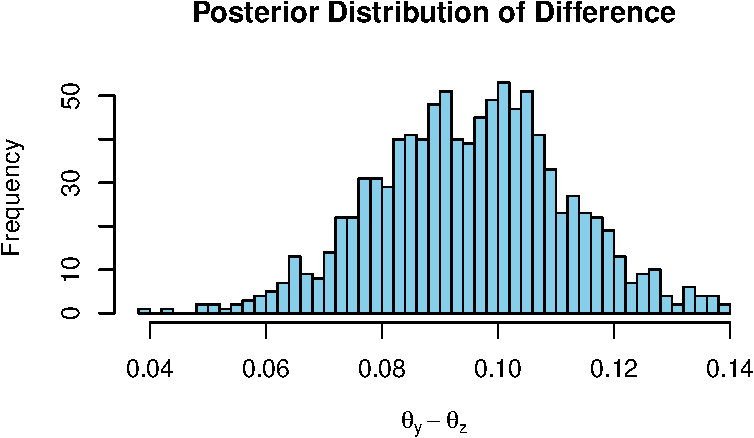
\includegraphics{551-HW-Q1_files/figure-pdf/unnamed-chunk-1-1.pdf}




\end{document}
